\chapter{使用方法}
\section{\LaTeX 环境}
本项目宏包依赖\LaTeXe 、Xe\TeX 以及C\TeX ,因此在使用前请确保这些发行版已经安装妥当。
本人在 MacTex2015 + OSX10.11 环境下运行通过。文件使用UTF-8编码,并使用 Xe\LaTeX 进行编译。

\section{目录结构}
项目目录由以下文件构成:
\begin{itemize}
\item \textcolor{blue}{main.tex} - 论文的基本骨架,你可以在此添加你需要的其他宏包
\item \textcolor{blue}{Makefile} - 在*nix(Linux/Mac OS X)环境下,使用 \verb|make| 命令完成论文的整体编译
\item \textcolor{blue}{scuthesis.sty} - 论文格式样式包,可以无视这个文件
\item \textcolor{blue}{src/info.tex} - 包含了作者基本信息
\item \textcolor{blue}{src/abstract.tex} - 包含了封面、中英文摘要以及目录的定义
\item \textcolor{blue}{src/ackno.tex} - 这个文件包含了论文参考文献、附录等信息
\item \textcolor{blue}{src/ch*.tex} - 论文每一章节的具体内容
\item \textcolor{blue}{src/table/data.csv} - 给出了从 CSV 文件导入表格的示例
\item \textcolor{blue}{src/img/pic.jpg} - 给出了导入图片的示例
\item \textcolor{blue}{src/code/main.c} - 给出了从文件导入代码的示例
\item \textcolor{blue}{src/ref/refs.bib} - bibtex 文献库,推荐使用 \href{http://jabref.sourceforge.net/}{JabRef} 维护
\end{itemize}

\section{如何使用}
本文将给予你一个粗略的使用本模版的示例。
\subsection{基本信息}
在 info.tex 文件中输入自己的基本信息。然后论文的摘要可以在 abstract.tex 中输入。同时,英文摘要也可以写在其中。
你可能需要包含自己的宏包,那么你可以在 main.tex 中添加 usepackag 命令。

\subsubsection{多级标题}
另外,随着章节数目增多,可以自行新建 ch*.tex 文件,并将其在 main.tex 中用 include 指令包含进来。最后,为了编译你的论文,你需要使用 xelatex 命令。

\section{注意事项}
\begin{enumerate}
\item 中英文摘要分别不能超过一页,否则第二页的板式会有错误。
\item 所有文件必须是 UTF-8 编码,否则编译不能通过。
\end{enumerate}

\section{插入资源}
这一节内容将向你展示如何插入图片、表格、公式及代码资源。
\subsection{插入图片}
毫无疑问,你肯定需要插入各种各样的图片,下面的图\ref{fig:one}是一个插入图片的例子。

\begin{figure}[htbp!]
\centering
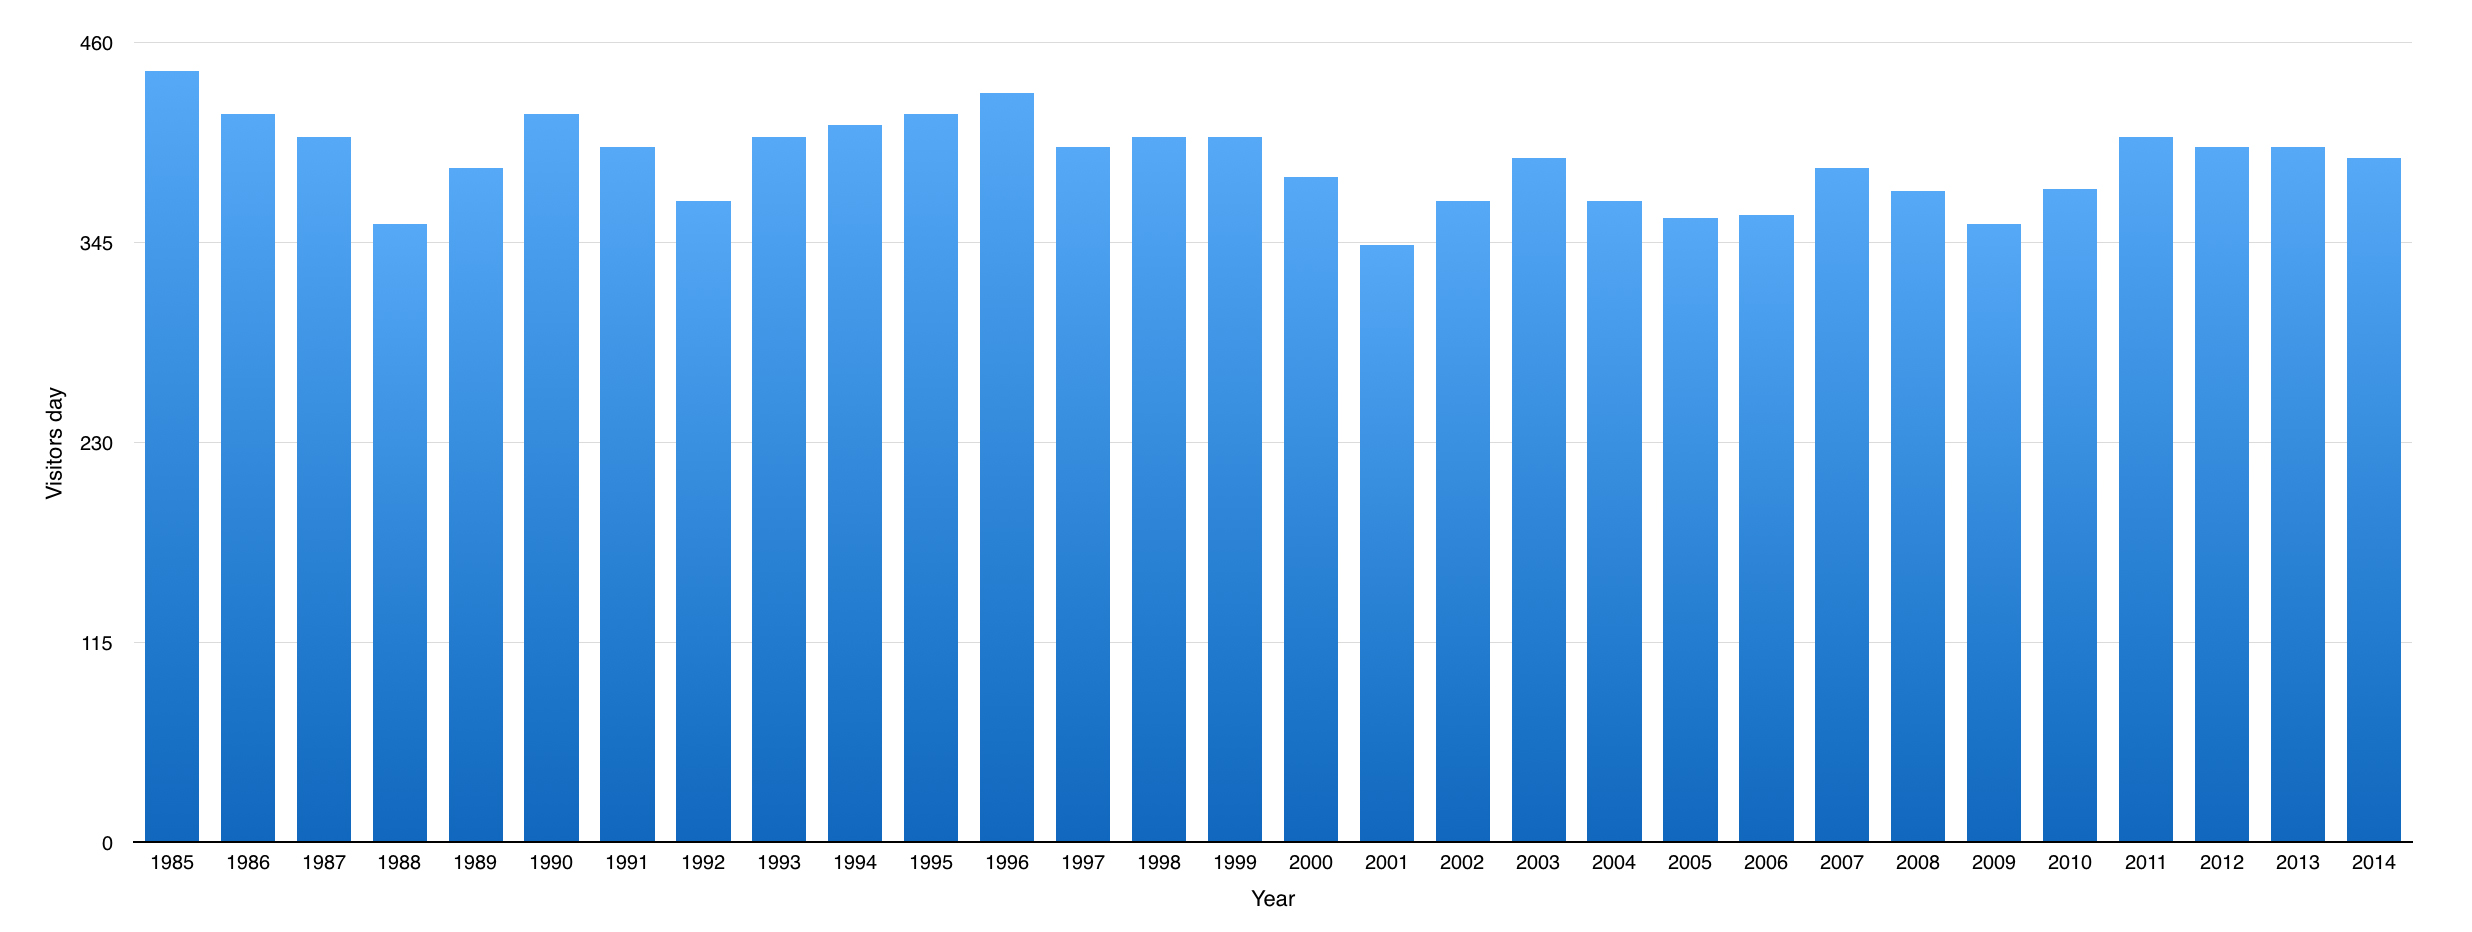
\includegraphics[scale=0.3]{src/img/pic.jpg} 
\caption{这是一张图片}\label{fig:one}
\end{figure}

当然插入图片你可能还会有其他需求,所以你可以参考一些网上的其他例子,但是就目前这个例子而言已经足够了。

\subsection{插入表格}
可能你还需要插入表格,表\ref{table:one}就是一个例子。

\begin{table}[htbp!]
\centering
\caption{这是一张表格}\label{table:one}\par
\csvautobooktabular{src/table/data.csv}
\end{table}

\subsection{插入公式}

下面则是一个很好的公式混排的例子。

设函数集$Q(z,\alpha ),\alpha \in \Lambda$满足条件

\begin{equation}
A\leq \int_{}^{}Q(z,\alpha ) dF(z)\leq B(A\leq R(\alpha)\leq B),
\end{equation}

那么EMR原则一致性的充分必要条件是:经验风险 $R_{emp}(\alpha)$ 在函数集$ Q(z,\alpha )\in \Lambda $上以如下意义一致收敛于期望风险 $R\left( \alpha \right)$

\begin{equation}
\lim_{l\rightarrow\infty}P \{ \sup_{\alpha\in\Lambda}(R(\alpha)-R_{emp}(\alpha))>\epsilon \}=0,\forall \epsilon>0
\end{equation}

\subsection{插入代码}
如果你是学计算机的,很明显你需要往文章中插入代码,所以,下面的代码展示了如何从文件中插入代码\ref{code:one}。
\lstinputlisting[
	language={[ANSI]C},
	morekeywords={World},
	emph={printf},
	title={代码\ref{code:one}:这段C语言代码的输出结果为 Hello World!\label{code:one}}
]{src/code/main.c}



